\documentclass[11pt]{article}
\usepackage[margin=1in]{geometry}
\usepackage[T1]{fontenc}
\usepackage{lmodern}
\usepackage{microtype}
\usepackage{amsmath,amssymb}
\usepackage{booktabs}
\usepackage{placeins}
\usepackage{xcolor}
\usepackage{tikz}
\usetikzlibrary{positioning,arrows.meta}
\usepackage[hidelinks]{hyperref}
\usepackage[numbers,sort&compress]{natbib}

\newcommand{\bgkit}{\textsc{bgkit}}

\title{\bgkit: Reading Compressed Context through\\a Language Model's Embedding Layer}
\author{Gabriel Pickard}
\date{October 2026}

\begin{document}
\maketitle

\begin{abstract}
\bgkit{} gives a language model access to far more text than fits in its context budget. A
bidirectional encoder reads a text together with a prompt that states what the reader needs, compresses
it by a chosen ratio, and projects the result into the decoder's input embedding space, where the
decoder reads it in place of the text's tokens. Any number of such compressed slots can be mixed with
ordinary text, and the same interface carries documents, tool results, conversation histories and
repositories. We train a 350M-parameter encoder with a 350M-parameter decoder on a single workstation
GPU and evaluate the system at a fixed number of decoder positions. With 2{,}048 positions the decoder
answers questions over 59k-token stories and 111k-token conversation histories, which it would
otherwise have to read in full or truncate to 2{,}048 tokens. In 25 of 26 settings across nine long-context benchmarks the compressed context
scores at least as high as the same decoder reading the text truncated to the same budget, for example
0.74 against 0.12 on BABILong with 15k-token contexts in 1{,}024 positions. On HotpotQA it also scores
above question-focused summaries written by a 35B-parameter model (0.64 against 0.55). On MuSiQue and
LoCoMo, which were not used in training, it scores above the original decoder reading the entire
context (0.30--0.33 against 0.13, and 0.28 against 0.19). Within a model, raising the compression from
4$\times$ to 64$\times$ costs little. Exact strings are not preserved: on RULER the full context
scores 0.58 and the compressed context 0.20. An agent that receives every tool result in compressed
form runs SWE-bench Lite localisation and web-research episodes end to end, with fewer decoder tokens
than when it reads text.
\end{abstract}

\section{Introduction}

A language model can use only what fits in its context window. Retrieved documents, tool output,
earlier conversation and source code compete for the same positions, and every position costs a full
pass through the model. Vision--language models handle a similar problem for images: a separate
encoder turns many pixels into a few vectors, which are projected into the language model's
token-embedding space and read like tokens \citep{alayrac2022flamingo,liu2023llava}.

\bgkit{} applies this to text. An encoder reads a text together with a prompt that states what the
reader needs from it, for example \emph{``answer: who founded the company?''} or \emph{``lines 80--140
of \texttt{io.py}: where is the buffer flushed?''}, and emits a short sequence of vectors in the
decoder's input embedding space. The decoder reads them in a slot in place of the text
(Figure~\ref{fig:arch}). The compression ratio is chosen per slot at inference time, and an input can
hold any number of slots alongside ordinary text. Because the slots are vectors in the decoder's own
embedding space, the encoder can also read its own output, which lets it summarise directory trees and
long histories hierarchically.

The paper makes three contributions:
\begin{itemize}
\item \textbf{A method} (Sections~\ref{sec:method}--\ref{sec:training}): the encoder, projection and
  slot interface, the training recipe, and an agent harness in which every tool result arrives
  compressed.
\item \textbf{Measurements of context savings} (Sections~\ref{sec:sweep}--\ref{sec:ratio}): on nine
  long-context benchmarks at a fixed decoder budget, compared with truncated text, question-focused
  summaries from a much larger model, and the original decoder reading the whole context; and the
  loss on held-out answers as the compression ratio grows.
\item \textbf{An agent that reads only compressed context} (Section~\ref{sec:agents}): SWE-bench Lite
  bug localisation, web research and conversational memory.
\end{itemize}
Section~\ref{sec:ablation} reports which parts of the encoder the results depend on.

\begin{figure}[t]
\centering
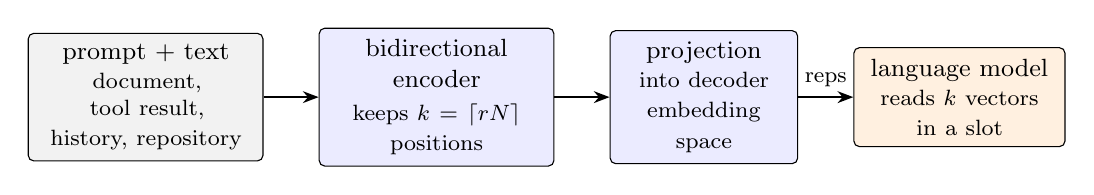
\begin{tikzpicture}[
  font=\small, node distance=7mm,
  box/.style={draw, rounded corners=2pt, align=center, minimum height=11mm, inner sep=4pt},
  ar/.style={-{Stealth[length=2mm]}, thick}]
  \node[box, fill=gray!10, text width=27mm] (in) {prompt + text\\[1pt]\footnotesize document, tool result,\\ history, repository};
  \node[box, fill=blue!8, text width=27mm, right=of in] (enc) {bidirectional encoder\\[1pt]\footnotesize keeps $k=\lceil rN\rceil$ positions};
  \node[box, fill=blue!8, text width=21mm, right=of enc] (proj) {projection\\[1pt]\footnotesize into decoder\\ embedding space};
  \node[box, fill=orange!12, text width=24mm, right=of proj] (dec) {language model\\[1pt]\footnotesize reads $k$ vectors\\ in a slot};
  \draw[ar] (in) -- (enc);
  \draw[ar] (enc) -- (proj);
  \draw[ar] (proj) -- node[above, font=\footnotesize] {reps} (dec);
\end{tikzpicture}
\caption{The \bgkit{} interface. An encoder reads a text under a prompt and emits $k$ vectors
(``reps'') in the decoder's embedding space. The decoder reads them in a slot among ordinary tokens;
one input can contain many slots.}
\label{fig:arch}
\end{figure}

\section{Method}
\label{sec:method}

\paragraph{Encoder.}
The encoder is LFM2.5-Encoder-350M, a 16-layer bidirectional model with hidden size 1024. Its input
is a prompt, a separator and the text to encode, so every text position can attend to the prompt.

\paragraph{Compression.}
After the middle layer, a scoring head ranks the text positions, and the top $k=\lceil rN\rceil$ of
the $N$ positions are kept for a compression ratio $r$. The remaining layers still run over the
whole sequence, so each kept position can gather information from anywhere in the text. The final
hidden states at the kept positions form the encoding. The ratio is a free parameter at inference
time: the same weights produce 4$\times$, 16$\times$ or 128$\times$ encodings.

\paragraph{Projection.}
A projection stage (an attention layer over the kept positions followed by an MLP) maps the encoding
into the decoder's input embedding space. A normalisation layer then matches the per-channel
statistics of the decoder's token embeddings. We added it after observing, in earlier versions, that
the projected vectors could collapse onto a shared direction while keeping a plausible norm.

\paragraph{Decoder.}
The decoder is LFM2.5-350M (instruction-tuned), and its input is rendered with its own chat template.
Each slot is marked by a placeholder token that is replaced by the slot's vectors, and an input may
contain any number of slots interleaved with text. A rank-32 low-rank adapter on the decoder's first
eight layers is trained to read the slots. The adapter applies at all positions, so it also changes
how the decoder reads ordinary text.

\paragraph{Hierarchical encodings.}
Because the vectors live in the decoder's embedding space, the encoder can also be applied to its
own output. We use this in three places:
\begin{itemize}
\item \emph{Repositories} are encoded bottom-up. Each file is encoded at 8$\times$, and each directory
  encodes its children's vectors at a further 4$\times$, up to a root \emph{overview} of a few
  hundred vectors. Nodes are cached and can be opened with a \texttt{browse} tool.
\item \emph{Long histories} are compacted by folding older turns into cells encoded at 16$\times$.
  Cells merge pairwise at 4$\times$, so the compacted history grows roughly logarithmically.
\item \emph{Conversational memory} is a set of per-session encodings with a compact index of all
  sessions. A session can be re-read under a new prompt.
\end{itemize}
The evaluations below exercise the repository overview and the memory index. History compaction is
not evaluated separately.

\paragraph{Agent harness.}
In our agent harness, file reads, code search, shell output, web search, page reads, find-in-page and
memory lookups all return slots rather than text. Each slot is encoded under the agent's own
statement of what it is looking for. Tools have fixed compression ratios: 4$\times$ for search hits
and find-in-page, where answers are often copied verbatim; 8$\times$ for file reads; 16$\times$ for
other search, shell output and page reads; 32$\times$ for the repository overview and compacted
history.

\section{Training}
\label{sec:training}

\paragraph{Objectives.}
The decoder is trained to produce a target (an answer, an agent's next turn, or a continuation of
the text) from an input in which the context appears only as encoded vectors. Three further signals
are added to this cross-entropy loss:
\begin{itemize}
\item \emph{Distillation from a full-text reader.} A decoder with a separately trained adapter reads
  the same input with the context as plain text, and the model reading encodings is trained to match
  its next-token distribution.
\item \emph{Prompt contrast.} A document is also encoded under a different question about it, and the
  correct answer is trained to be more likely under the right prompt than under the wrong one.
\item \emph{Preservation.} On a stream of ordinary chat and long-text reading, the adapted decoder is
  distilled towards the original decoder, to limit damage to its general behaviour.
\end{itemize}
The scoring head receives a small auxiliary loss that pushes it to follow the full-text reader's
attention from the answer to the context.

\paragraph{Compression curriculum.}
Each example's ratio is sampled between 4$\times$ and a floor that moves from 64$\times$ towards
128$\times$ during training. In agent data, tool slots use the harness ratios, randomly scaled by up
to a factor of two.

\paragraph{Data.}
Training mixes reconstruction and continuation of plain text (web text, code, books, dialogue) with
task data rendered as conversations whose contexts become slots:
\begin{itemize}
\item reading comprehension and long-document QA, including the training splits of HotpotQA, QuALITY
  and NarrativeQA (benchmark-test stories excluded);
\item bAbI tasks 1--3 (training split) hidden in book, web and wiki filler, which is how BABILong
  builds its test set;
\item multi-hop QA with distractors and synthetic needle retrieval;
\item agent trajectories on software repositories (generated by a larger teacher model and
  rejection-sampled), with repository QA, file localisation and repository overviews;
\item web-research trajectories mapped onto the web tools;
\item multi-session conversations (from MSC, Chronicles and SHARE) with generated questions about
  their history.
\end{itemize}
No evaluation item appears in training. BABILong, HotpotQA, QuALITY and NarrativeQA are therefore
in-distribution task formats; MuSiQue, RULER, LongMemEval and LoCoMo were used only for evaluation.

\paragraph{Parameters and compute.}
In the final stages the base encoder weights are frozen. A rank-16 adapter on its top four layers,
the scoring head and the projection are trained, together with the decoder adapter. All training ran
on a single NVIDIA DGX Spark. The evaluated checkpoint ends a chain of warm-started development runs:
its final three stages took 40{,}000 steps (8{,}000, 12{,}000 and 20{,}000), with the agentic, web
and memory data at full weight in the last 20{,}000. The encoder and adapters inherit weights from
earlier runs on overlapping data.

\section{Evaluation setup}
\label{sec:setup}

Every benchmark comparison uses a fixed \emph{budget}: the number of decoder positions the context may
occupy. The arms are:
\begin{description}
\item[bgkit] The context is compressed to fit the budget, with the question as the encoder prompt.
\item[text] The same trained decoder reads the context as text, middle-truncated to the budget.
\item[base] The original decoder (adapter off) reads the same truncated text.
\item[summary] Qwen3.6-35B-A3B writes a question-focused summary at the budget, which the trained
  decoder reads as text. For HotpotQA the summariser reads about 1{,}600 tokens and generates about
  280 per item. This arm was run for some budgets only.
\item[base, full context] The original decoder reads the whole context without truncation. This arm
  is not budget-matched.
\end{description}
The trained decoder was trained to read compressed slots, not to answer from text, so the \emph{text}
arm uses it outside its training distribution. The encoder sees the question and truncation does not;
the \emph{summary} arm is the question-aware text baseline.

BABILong \citep{kuratov2024babilong} (tasks qa1--qa3), RULER \citep{hsieh2024ruler} and QuALITY
\citep{pang2022quality} are scored by accuracy. NarrativeQA \citep{kocisky2018narrativeqa}, HotpotQA
\citep{yang2018hotpotqa}, MuSiQue \citep{trivedi2022musique}, LongMemEval \citep{wu2025longmemeval}
and LoCoMo \citep{maharana2024locomo} are scored by an LLM judge (Qwen3.6-35B-A3B). Cells have 60--100
items, so an accuracy near 0.5 carries a 95\% interval of about $\pm0.1$.

\section{Long contexts at a fixed budget}
\label{sec:sweep}

Table~\ref{tab:sweep} reports the nine benchmarks. Contexts range from 1.4k tokens (HotpotQA) to
111k (LongMemEval-S), and budgets from 256 to 8{,}192 positions, so the compression ratio ranges from
under 2$\times$ to about 54$\times$.

\begin{table}[p]
\centering
\small
\begin{tabular}{llrrrr|r}
\toprule
Benchmark ($n$) & Budget & bgkit & text & base & summary & \shortstack{base,\\full context} \\
\midrule
BABILong 16k (100) & 1,024 & \textbf{0.74} & 0.12 & 0.08 & -- & 0.18 \\
\quad 15.4k tokens & 2,048 & \textbf{0.76} & 0.19 & 0.13 & -- &  \\
 & 4,096 & \textbf{0.74} & 0.22 & 0.13 & -- &  \\
\midrule
BABILong 4k (100) & 512 & \textbf{0.79} & 0.20 & 0.16 & 0.31 & 0.27 \\
\quad 3.6k tokens & 1,024 & \textbf{0.81} & 0.26 & 0.23 & 0.23 &  \\
 & 2,048 & \textbf{0.88} & 0.33 & 0.21 & -- &  \\
\midrule
RULER 4k (100) & 512 & \textbf{0.20} & 0.09 & 0.07 & -- & 0.58 \\
\quad 3.7k tokens & 1,024 & \textbf{0.20} & 0.15 & 0.11 & -- &  \\
 & 2,048 & 0.17 & 0.22 & \textbf{0.24} & -- &  \\
\midrule
QuALITY (100) & 512 & 0.36 & 0.31 & 0.25 & \textbf{0.42} & 0.31 \\
\quad 6.0k tokens & 1,024 & \textbf{0.36} & 0.33 & 0.27 & -- &  \\
 & 2,048 & 0.37 & 0.34 & 0.26 & \textbf{0.45} &  \\
\midrule
NarrativeQA (60) & 2,048 & \textbf{0.17} & 0.07 & 0.05 & -- & -- \\
\quad 58.6k tokens & 4,096 & \textbf{0.17} & 0.10 & 0.10 & -- &  \\
 & 8,192 & \textbf{0.15} & 0.12 & 0.08 & -- &  \\
\midrule
HotpotQA (100) & 256 & \textbf{0.64} & 0.23 & 0.25 & 0.55 & 0.45 \\
\quad 1.4k tokens & 512 & \textbf{0.62} & 0.35 & 0.27 & 0.53 &  \\
 & 1,024 & \textbf{0.60} & 0.37 & 0.39 & -- &  \\
\midrule
MuSiQue (100) & 512 & 0.30 & 0.08 & 0.08 & \textbf{0.42} & 0.13 \\
\quad 2.5k tokens & 1,024 & 0.31 & 0.08 & 0.10 & \textbf{0.40} &  \\
 & 2,048 & \textbf{0.33} & 0.16 & 0.10 & -- &  \\
\midrule
LongMemEval-S (60) & 2,048 & \textbf{0.30} & 0.18 & 0.10 & -- & -- \\
\quad 110.7k tokens & 4,096 & \textbf{0.23} & 0.15 & 0.05 & -- &  \\
 & 8,192 & \textbf{0.20} & 0.15 & 0.02 & -- &  \\
\midrule
LoCoMo (100) & 1,024 & \textbf{0.28} & 0.09 & 0.08 & -- & 0.19 \\
\quad 18.8k tokens & 2,048 & \textbf{0.28} & 0.16 & 0.13 & -- &  \\
\bottomrule
\end{tabular}

\caption{Accuracy by benchmark and budget (decoder positions available to the context); the second
line of each benchmark gives its mean context length. BABILong, RULER and QuALITY: accuracy; the
others: LLM-judge accuracy. Bold: best budget-matched arm. Summaries were generated for a subset of
budgets (QuALITY summaries for 60 and 56 items). The last column is the original decoder reading the
whole, untruncated context on the same items and is not budget-matched; it was not run for
LongMemEval-S (contexts above the 32k-token limit of our full-context runs) and has too few shared
items for NarrativeQA.}
\label{tab:sweep}
\end{table}

\paragraph{Against truncated text.}
In 25 of 26 benchmark--budget cells the compressed context scores at least as high as the same
decoder reading truncated text; the exception is RULER at 2{,}048 positions. The largest margins are
on contexts much longer than the budget: BABILong 16k (0.74--0.76 against 0.12--0.22), LoCoMo (0.28
against 0.09--0.16), and NarrativeQA (0.15--0.17 against 0.07--0.12, on stories averaging 59k
tokens).

\paragraph{Against a larger model's summaries.}
On HotpotQA the compressed context scores above question-focused summaries written by
Qwen3.6-35B-A3B at both budgets where both were run (0.64 against 0.55 at 256 positions, 0.62 against
0.53 at 512). The summaries score higher on MuSiQue (0.40--0.42 against 0.30--0.31) and QuALITY
(0.42--0.45 against 0.36--0.37); BABILong 4k is split. The encoder needs one forward pass of a 350M
model; each summary is generated token by token by a mixture-of-experts model with 3B active
parameters.

\paragraph{Against the full context.}
On MuSiQue and LoCoMo, which were not used in training, the compressed context scores above the
original decoder reading the entire context: 0.30--0.33 against 0.13, and 0.28 against 0.19. The
same holds on BABILong (0.74 against 0.18) and HotpotQA (0.64 against 0.45), whose task formats were
in training. Part of these margins therefore comes from training on reading tasks rather than from
compression itself; what they show about compression is that the compressed context retains what
these questions need.

\paragraph{Exact strings.}
RULER's needle tasks, also not used in training, ask for exact keys and numbers. Here the full
context scores 0.58 and the compressed context 0.17--0.20: arbitrary strings are not preserved at these
ratios. The agent harness accordingly reads search hits at only 4$\times$.

\paragraph{Conversation histories.}
On LongMemEval-S (111k tokens per history) the compressed context scores 0.20--0.30 against
0.15--0.18 for truncated text, with the highest score at the smallest budget.


\section{Compression ratio}
\label{sec:ratio}

Table~\ref{tab:ratio} gives the decoder's loss on the gold answer at four compression ratios, on
held-out items from three training task families and an earlier checkpoint of the same model. From
4$\times$ to 64$\times$ the loss rises by 0.12--0.19 nats, while removing the context costs 1.9--3.3
nats. At 128$\times$ the loss rises further on SQuAD and bAbI-in-filler (to 1.04 and 0.84 nats). The
benchmarks show the same pattern where the budget varies the ratio: BABILong 16k scores 0.74--0.76 from
about 4$\times$ to 15$\times$, and NarrativeQA 0.15--0.17 from about 7$\times$ to 29$\times$.

\begin{table}[!ht]
\centering
\small
\begin{tabular}{lrrrr|r}
\toprule
Task & 4$\times$ & 16$\times$ & 64$\times$ & 128$\times$ & no context \\
\midrule
SQuAD & 0.40 & 0.43 & 0.59 & 1.04 & 2.30 \\
Multi-needle & 0.47 & 0.58 & 0.59 & 0.66 & 3.01 \\
bAbI-in-filler & 0.22 & 0.14 & 0.35 & 0.84 & 3.48 \\
\bottomrule
\end{tabular}

\caption{Decoder loss on the gold answer (nats per token) by compression ratio: held-out items of
three training task families (96 each), earlier checkpoint, question as the encoder prompt.}
\label{tab:ratio}
\end{table}

\section{Agentic tasks}
\label{sec:agents}

Agent evaluations run the full harness with at most 12 turns and 40{,}000 decoder tokens per episode.
In the \emph{text} arms, tool results are returned as text cut to the same per-result budget. The
policy was trained on episodes with compressed tool results, so the text arms run it outside its
training distribution.

\paragraph{Bug localisation.}
On SWE-bench Lite \citep{jimenez2024swebench} the agent starts from the issue and the repository at
its base commit, explores, and names the file to change. We excluded the 114 Django instances, whose
repository trees exceeded our caching limit, leaving 186 (Table~\ref{tab:swe}). With the repository
overview, a few hundred vectors standing for the whole tree, in its context, the agent commits to an
answer in 59\% of episodes instead of 22\%, never ends in a loop (70\% without it), and uses 13.9k
instead of 19.5k decoder tokens. It names a file edited by the reference patch in 14 of 186 episodes
(7.5\%; 95\% interval about 4.5--12\%), against 1 for the text agent with the same overview. The
agent made no \texttt{browse} calls, so this measures the root overview alone.

\begin{table}[!ht]
\centering
\small
\begin{tabular}{lrrrrrr}
\toprule
Arm & \shortstack{Gold file\\named} & \shortstack{Gold file\\opened} & Answered & Turns & Looped & \shortstack{Decoder\\tokens} \\
\midrule
bgkit + overview & 0.075 (14) & 0.086 & 0.59 & 3.9 & 0.00 & 13.9k \\
bgkit & 0.027 (5) & 0.118 & 0.22 & 7.1 & 0.70 & 19.5k \\
text + overview & 0.005 (1) & 0.011 & 0.04 & 2.3 & 0.00 & 21.6k \\
text & 0.000 (0) & 0.005 & 0.02 & 2.6 & 0.02 & 22.7k \\
\bottomrule
\end{tabular}

\caption{Bug localisation on SWE-bench Lite without Django (186 instances). Gold file named: the final
answer names a file edited by the reference patch (count in parentheses). Answered: the episode ends
with a file answer. Looped: the episode was stopped for a repeated call. Decoder tokens: per
episode.}
\label{tab:swe}
\end{table}

\paragraph{Web research.}
The agent searches a BM25 index, opens pages and finds passages, with every result compressed
(Table~\ref{tab:web}). On HotpotQA questions searched over the pool of 87{,}593 validation paragraphs,
judge accuracy is 0.27 against 0.14 for the text agent, with 2.4k instead of 6.5k decoder tokens per
episode and loops in 4\% of episodes instead of 43\%. On MuSiQue both arms are near zero (0.05 and
0.03), and on BrowseComp-Plus \citep{chen2025browsecompplus} neither answers any question.

\begin{table}[!ht]
\centering
\small
\begin{tabular}{llrrrrr}
\toprule
Benchmark & Arm & Judge acc. & EM & Turns & Looped & \shortstack{Decoder\\tokens} \\
\midrule
HotpotQA (pool) & bgkit & 0.27 & 0.16 & 2.7 & 0.04 & 2.4k \\
 & text & 0.14 & 0.11 & 6.1 & 0.43 & 6.5k \\
\midrule
MuSiQue (pool) & bgkit & 0.05 & 0.01 & 3.1 & 0.02 & 3.3k \\
 & text & 0.03 & 0.03 & 6.3 & 0.44 & 7.2k \\
\midrule
BrowseComp-Plus & bgkit & 0.00 & 0.00 & 2.1 & 0.05 & 3.0k \\
 & text & 0.00 & 0.00 & 2.3 & 0.10 & 3.4k \\
\bottomrule
\end{tabular}

\caption{Web research (100 questions each). HotpotQA and MuSiQue search the pooled paragraphs of
their validation sets; BrowseComp-Plus searches its fixed web corpus.}
\label{tab:web}
\end{table}

\paragraph{Conversational memory.}
LongMemEval-S and LoCoMo were also run with a two-stage memory agent, which sees an index of sessions
compressed under a generic prompt and re-reads sessions under its own focus. It reaches judge accuracy
of 0.05 on LongMemEval-S and 0.06 on LoCoMo
\unskip, against 0.30 and 0.28 when every session is compressed under
the question (Table~\ref{tab:sweep}).

\section{What the encoding depends on}
\label{sec:ablation}

Table~\ref{tab:ablation} varies how the encoding is produced, on the items and checkpoint of
Table~\ref{tab:ratio}. Replacing the learned position selection with random positions of the same
number changes exact match little on SQuAD (0.61 in both) and lowers it on multi-needle (0.54 against
0.58) and bAbI-in-filler (0.82 against 0.90). Removing the prompt lowers exact match to 0.04--0.21.
With the prompt for a different question about the same document, the loss on the correct answer
exceeds the no-context loss on SQuAD (3.16 against 2.30 at 4$\times$) and multi-needle (4.32 against
3.01). The encoding is therefore specific to its prompt: an encoding made under one question can be
reused for another only when the prompt does not depend on the question, as for the repository
overview and the memory index.

\begin{table}[!ht]
\centering
\small
\resizebox{\linewidth}{!}{\begin{tabular}{lrrrrrrrrr}
\toprule
 & \multicolumn{3}{c}{SQuAD} & \multicolumn{3}{c}{Multi-needle} & \multicolumn{3}{c}{bAbI-in-filler} \\
\cmidrule(lr){2-4}\cmidrule(lr){5-7}\cmidrule(lr){8-10}
Encoder condition & EM & $\mathcal{L}_{4\times}$ & $\mathcal{L}_{64\times}$ & EM & $\mathcal{L}_{4\times}$ & $\mathcal{L}_{64\times}$ & EM & $\mathcal{L}_{4\times}$ & $\mathcal{L}_{64\times}$ \\
\midrule
question prompt, learned selection & 0.61 & 0.40 & 0.59 & 0.58 & 0.47 & 0.59 & 0.90 & 0.22 & 0.35 \\
question prompt, random selection & 0.61 & 0.43 & 0.59 & 0.54 & 0.51 & 0.67 & 0.82 & 0.20 & 0.61 \\
no prompt & 0.07 & 1.69 & 2.01 & 0.04 & 2.50 & 2.88 & 0.21 & 1.73 & 1.44 \\
prompt for a different question & 0.10 & 3.16 & 2.64 & 0.01 & 4.32 & 4.00 & 0.45 & 1.71 & 1.54 \\
\midrule
no context & -- & \multicolumn{2}{c}{2.30} & -- & \multicolumn{2}{c}{3.01} & -- & \multicolumn{2}{c}{3.48} \\
\bottomrule
\end{tabular}
}
\caption{Encoder conditions, same items and checkpoint as Table~\ref{tab:ratio}. EM: exact match of
generated answers at 64$\times$. $\mathcal{L}$: decoder loss on the gold answer (nats per token) at
4$\times$ and 64$\times$; lower is better. ``No context'' is the decoder's loss with the context
removed.}
\label{tab:ablation}
\end{table}

\section{Limitations}

\begin{itemize}
\item \textbf{Baselines.} The text arms use a decoder trained on compressed slots, not on text. A
  decoder fine-tuned on the same data with text contexts at the same budget, and question-aware token
  pruning \citep{jiang2024longllmlingua}, were not run.
\item \textbf{Task overlap.} The task formats of BABILong, HotpotQA, QuALITY and NarrativeQA are in
  training (their training splits, or bAbI's generator for BABILong). MuSiQue, RULER, LongMemEval and
  LoCoMo were not trained on.
\item \textbf{Scale and sample size.} Encoder and decoder have 350M parameters each, evaluation cells
  have 60--186 items, and the agentic results rest on small counts. We ran one seed.
\item \textbf{Encoder cost.} An encoding made under a question serves that question, so each new
  question needs a new encoder pass over the text. The savings reported here are in decoder
  positions; we did not measure end-to-end cost.
\item \textbf{Exact strings.} Arbitrary keys and numbers are lost at these ratios (RULER).
\item \textbf{Training history.} The evaluated model ends a chain of warm-started development runs,
  and the recipe has not been reproduced from scratch.
\end{itemize}

\section{Related work}

Prior work compresses context for language models in several ways: summary tokens the model learns
to write for itself \citep{mu2023gist,chevalier2023autocompressors}; autoencoders that produce memory
slots for a frozen decoder \citep{ge2024icae}; a single retrieval embedding projected into the decoder
\citep{cheng2024xrag}; context encoders read through cross-attention \citep{yen2024cepe}; and
dropping tokens, either independently of the question \citep{jiang2023llmlingua,pan2024llmlingua2}
or conditioned on it \citep{jiang2024longllmlingua}. Question-focused abstractive compression of
retrieved documents \citep{xu2024recomp} corresponds to our summary baseline. Vision--language models
connect separately trained encoders to language models through projections into the embedding space
\citep{alayrac2022flamingo,liu2023llava}. \bgkit{} combines a prompt-conditioned bidirectional encoder
with the decoder's embedding layer, applies it hierarchically to repositories and histories, and uses
it as the channel through which an agent receives all tool output.

\section{Conclusion}

\bgkit{} compresses text into vectors that a decoder reads through its embedding layer, under a prompt
that states what the reader needs. With a 350M encoder and a 350M decoder, a budget of a few thousand
positions gives the decoder access to contexts of tens to over a hundred thousand tokens. At equal
budget the compressed context scores above truncated text on almost all of the benchmarks we tested,
retains what multi-hop and conversational-memory questions need, and loses exact strings. The same
interface lets an agent work with every tool result in compressed form. Next steps are the baselines
listed above, encodings that can be reused across questions, and pairing a small encoder with a much
larger decoder.

\bibliographystyle{plainnat}
\bibliography{references}

\end{document}
